% Front Page
\title{Exam Time Table\\ Report}
\author{\textbf{Group 3} [MA-ZZ] \bigskip\\
        Jacopo Maggio\\Stefano Munna\\Jacopo Nasi\\Andrea Santu\\Marco Torlaschi}
\date{\bigskip\bigskip\today}

\documentclass[12pt]{article}
\usepackage[utf8]{inputenc}
\usepackage[italian]{babel}
\usepackage{geometry}
\usepackage{indentfirst}
\usepackage{mathtools}
\usepackage[usenames, dvipsnames]{color}
\usepackage{float}
\usepackage{amssymb}
\usepackage{ifsym}
% Measurement
\geometry{ a4paper, total={170mm,257mm},left=35mm, right=35mm, top=30mm, bottom=30mm }

\begin{document}

\begin{figure}
  \centering
  
\includegraphics[width=10cm]{images/polito.pdf}
\end{figure}

\maketitle % Print credits
\newpage

% Model pages
\section{Report}
This document provides some explanations about our solution to the proposed problem. The project has been developed in C with support of CLion (JetBrains IDE) and GitHub.
\\No external already implemented libraries have been used and a single thread approach has been chosen.

\subsection{Data Structures}
The main data structure is a graph, built on an adjacency matrix. Each element (e1,e2) of this matrix represents a relation of conflict between exam e1 and e2.It  can assume value:
\begin{equation}
  \begin{gathered}
    adjM_{e1,e2} = \begin{cases} 1 \rightarrow $ \textit{If \textbf{e1} and \textbf{e2}} can't be sustained in the same ts$ \\ -1 \rightarrow Otherwise \end{cases}
  \end{gathered}
\end{equation}
The choice over this structure is related to its ease and the fact that it allows a fast reading of the instances, a fast benchmark calculation and feasibility check.

\subsection{Workflow}
The first problem to be solved is to find a \textbf{feasible} solution to be used for the successive improvement.\\
Our approach consisted on splitting the problem in two parts:
\begin{enumerate}
  \item Find a solution without conflicts (also using a number of timeslots higher then those provided by  the instance).
  \item Elaborate with metaheuristics the previous unfeasible solution to obtain a feasible solution.
\end{enumerate}
The advantages of these implementations are the reduction of computational time and the easiness to implement it.

\paragraph{Greedy} The first phase, implemented by a greedy algorithm, tries to generate a feasible solution adding one exam at the time into the with the idea to reduce "the complexity" of the initial search.
The procedure works on a data structure of exams sorted by collision number (from exam with more collisions to the one whit fewer ones). The main steps are the following:
\begin{enumerate}
  \item Try to schedule each exam in the first available timeslot that not generate conflicts.
  \item If no timeslot is available, add a new timeslot.
\end{enumerate}
As we said, this first step can produce a solution that doesn't fit the instance requirements.
A first feasible solution (with the correct number of timeslots) is obtained after the next step.

\paragraph{Tabu Search} The goal of the second step is to reduce the number of added timeslots to the correct number,generating a feasible solution.
The workflow is:
\begin{enumerate}
  \item Decrease the number of timeslots of the previous produced solution by 1 until correct timeslot number is reached.
  \item Swap exams in a way to resolve conflicts (updating teh tabu list) and evaluate the solution.
  After all swaps:
  \item \begin{itemize}
    \item If no feasible solution has been found : Backtrack to solution with an extra timeslot.
    \item If a feasible solution has been found : Restart from point 1.
  \end{itemize}
\end{enumerate}
This procedure could have been used even without the aid of the previous step, but it would be too slow with high complexities of instances.

The second problem to be solved is to \textbf{improve} the found solution using some heuristic algorithms.\\
This task is fulfilled by four different procedures: \textit{LocalSearch, LocalSwap, SimulatedAnnealing and GreedySlotShuffle}.\\

The \textbf{LocalSearch} procedure works in three different ways:
\begin{itemize}
  \item \textbf{Move Exam}: Move an exam to another timeslot.
  \item \textbf{Swap Exam}: Swap exams scheduled in a time slot with those in another.
  \item \textbf{Bounded Shift}: Shift a portion of the timetable.
\end{itemize}

The \textbf{LocalSwap} procedure implements a steepest descent strategy and evaluates the Neighborhood \textit{N(x)} of the current optimal solution \textit{x}. The flow:
\begin{enumerate}
  \item Switches exams scheduled in a timeslot with those contained in any another to find a new feasible \textit{x'}.
  \item If \textit{x'} has a better benchmark than that of x, then \textit{x=x'}.
  \item Loop until no improvement.
\end{enumerate}
We have choose the ST strategy respect the first improvement due to its efficiency, despite its slower speed. All the local search and the local swap strategies are applied in loop until the solution is improving.\\

The \textbf{SimulatedAnnealing} procedure is used to avoid being stuck in a local minimum.
Our implementation is not different from the studied one. After some tuning we have used a starting temperature of 1000, that decrease of alfa = 0.9 every L = 10 iterations. After each temperature reduction,if an unfeasible solution has been produced as output, the feasability is restored using the tabu search and the minimum is searched using the local search.\\
Applying this algorithm, due to its randomness, could give different (even worst between different running) results.\\

The last implemented function is the \textbf{GreedySlotShuffle},a really simple algorithm that, starting from a feasible solution, swap timeslots randomly evaluating the benchmark.
\subsection{Other Solution}
Another tried, but not implemented, approach is the \textbf{Genetic}. We chose not to use it because it did not seem fit very well our implementation of the problem.

\subsection{Conclusions}
\paragraph{Problems}
The two main problems encountered in the design were:
\begin{enumerate}
  \item Search of the first feasible solution.
  \item Avoid being stuck in a local minimum.
\end{enumerate}
While the first problem has been completely solved, due to the randomness of the Simulated Annealing and the fact that, if an unfeasible solution is accepted, the tabu search is used to restore feasibility, sometimes the solver needs a consistent amount of time to escape a local minimum (as seen in the following graph).

\begin{figure}[H]
	\centering
	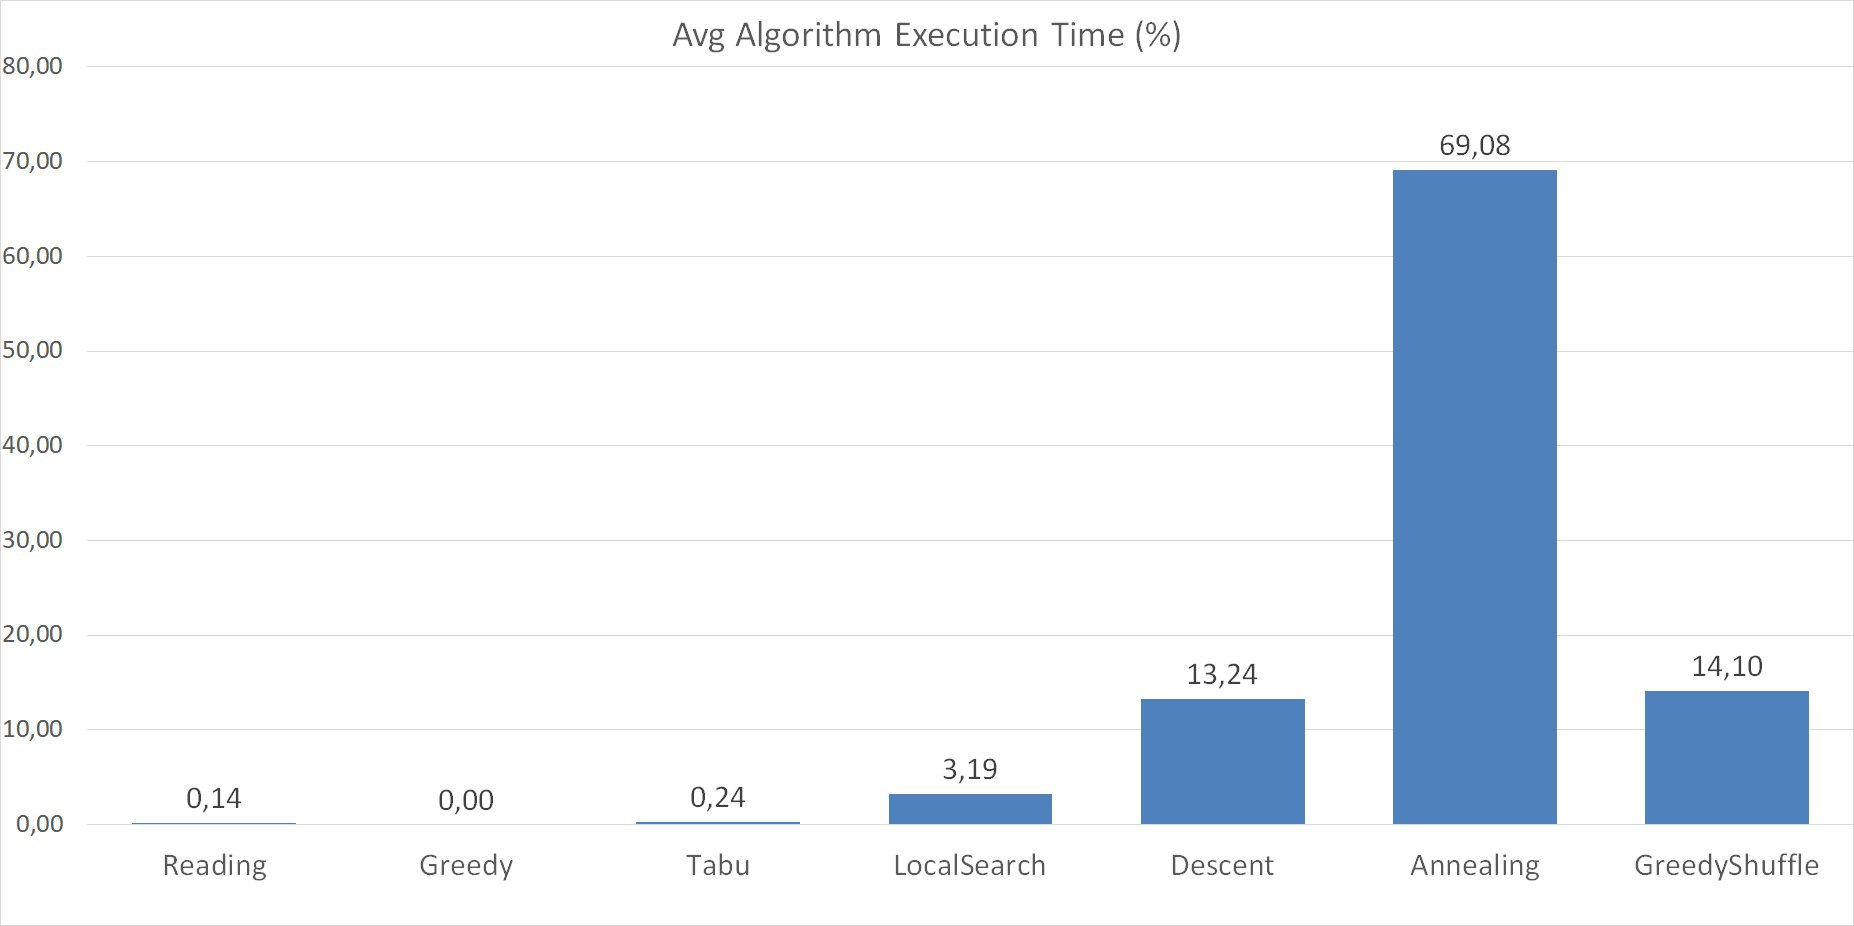
\includegraphics[width=\linewidth]{images/timeExec.jpg}
\end{figure}

\paragraph{Improvements}
To improve the performance of the solver, a multi-thread and a multi-start can be used.
\end{document}
